\subsubsection{\Cooperation}
\label{ssec:designdims:cooperation}

% <<<<<<< Updated upstream
% =======
% \begin{figure}[t]
%   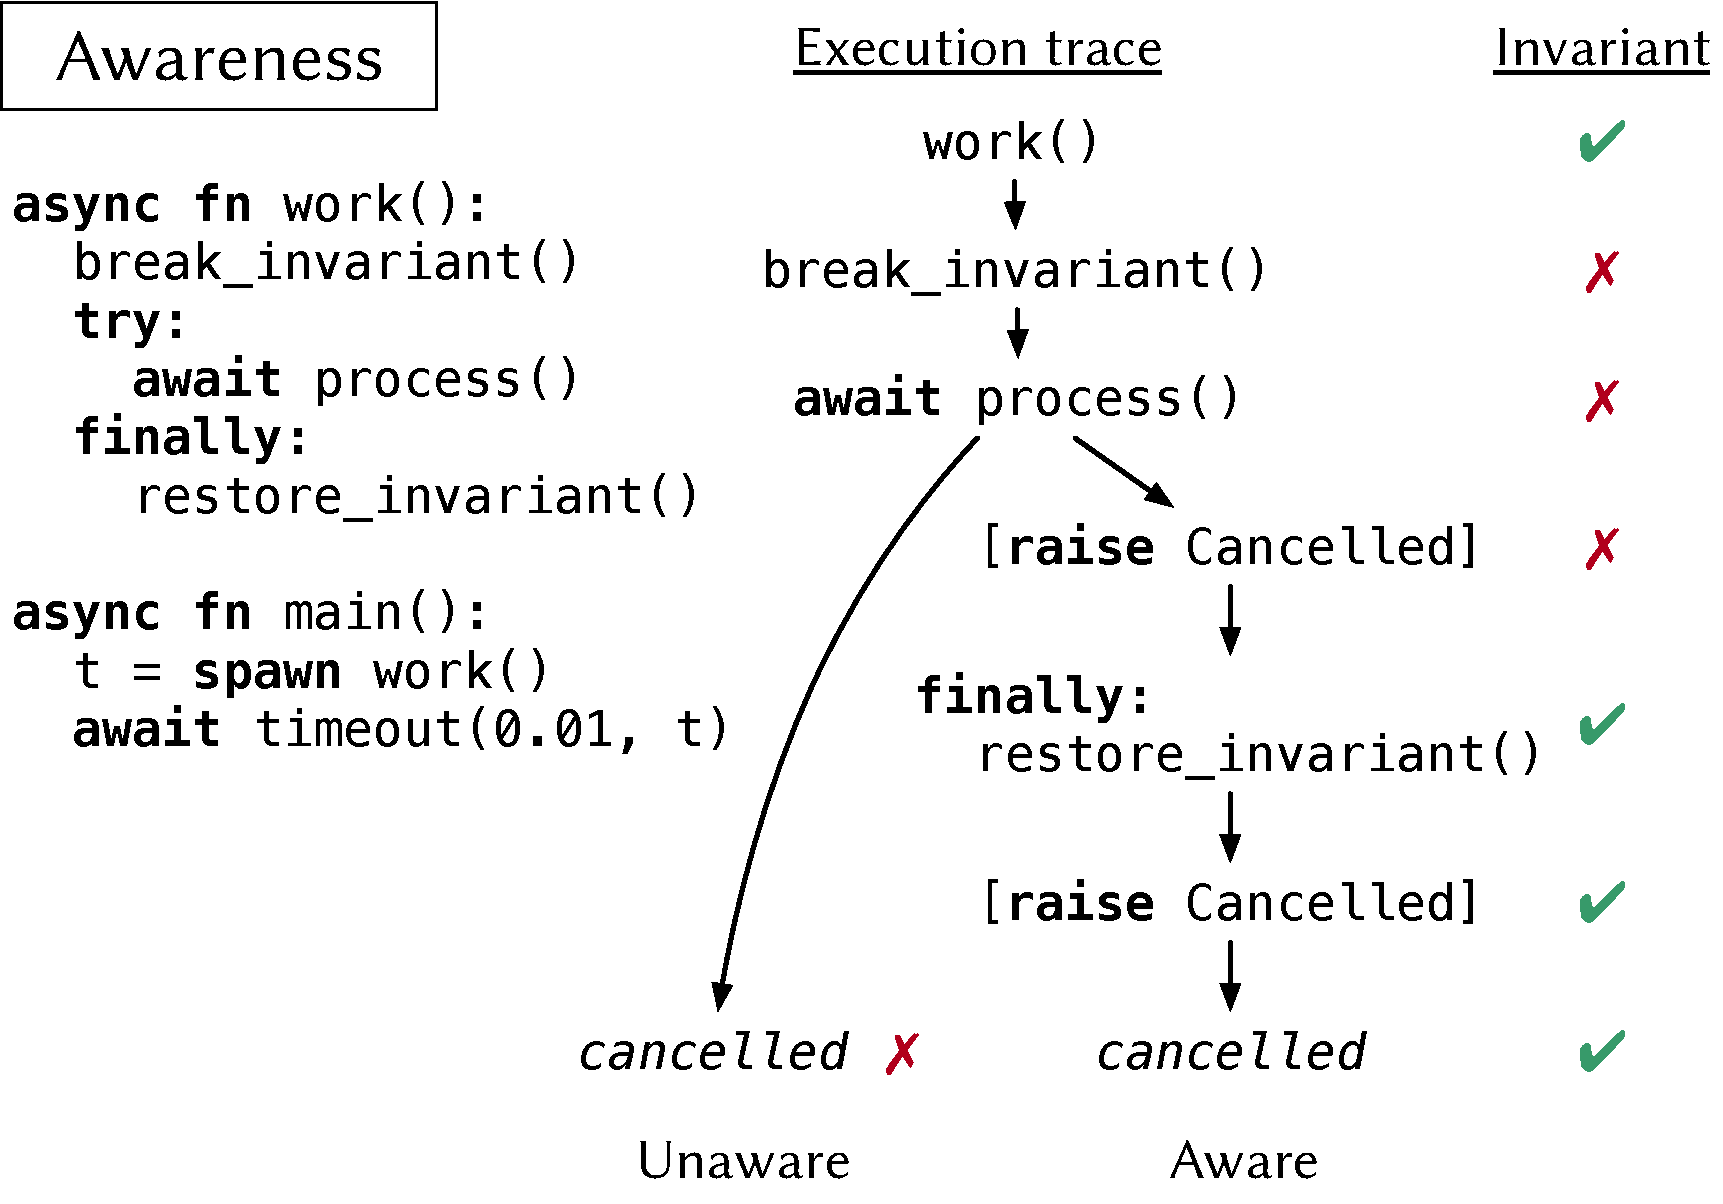
\includegraphics[width=0.85\linewidth]{f/cooperation.pdf}
%   \caption{An example program demonstrating the \Cooperation dimension. Each diagram shows the state, broken or intact, of a global invariant as the \code{work} task runs. Unaware cancellation does not communicate to the task that its being cancelled, leaving the invariant broken in this example. Aware cancellation provides a cancelled task the opportunity to handle cancellation, here the cancelled task reinstates the broken invariant before cancelling.}
%   \label{fig:cooperation}
% \end{figure}
% >>>>>>> Stashed changes
Integrated cancellation approaches all center around triggering cancellations at await points. A key distinction is whether a cancelled task is aware that it is being cancelled, in order to handle or ignore the cancellation at a given await point. 

\begin{wrapfigure}{r}{0.6\linewidth}
% \begin{figure*}
  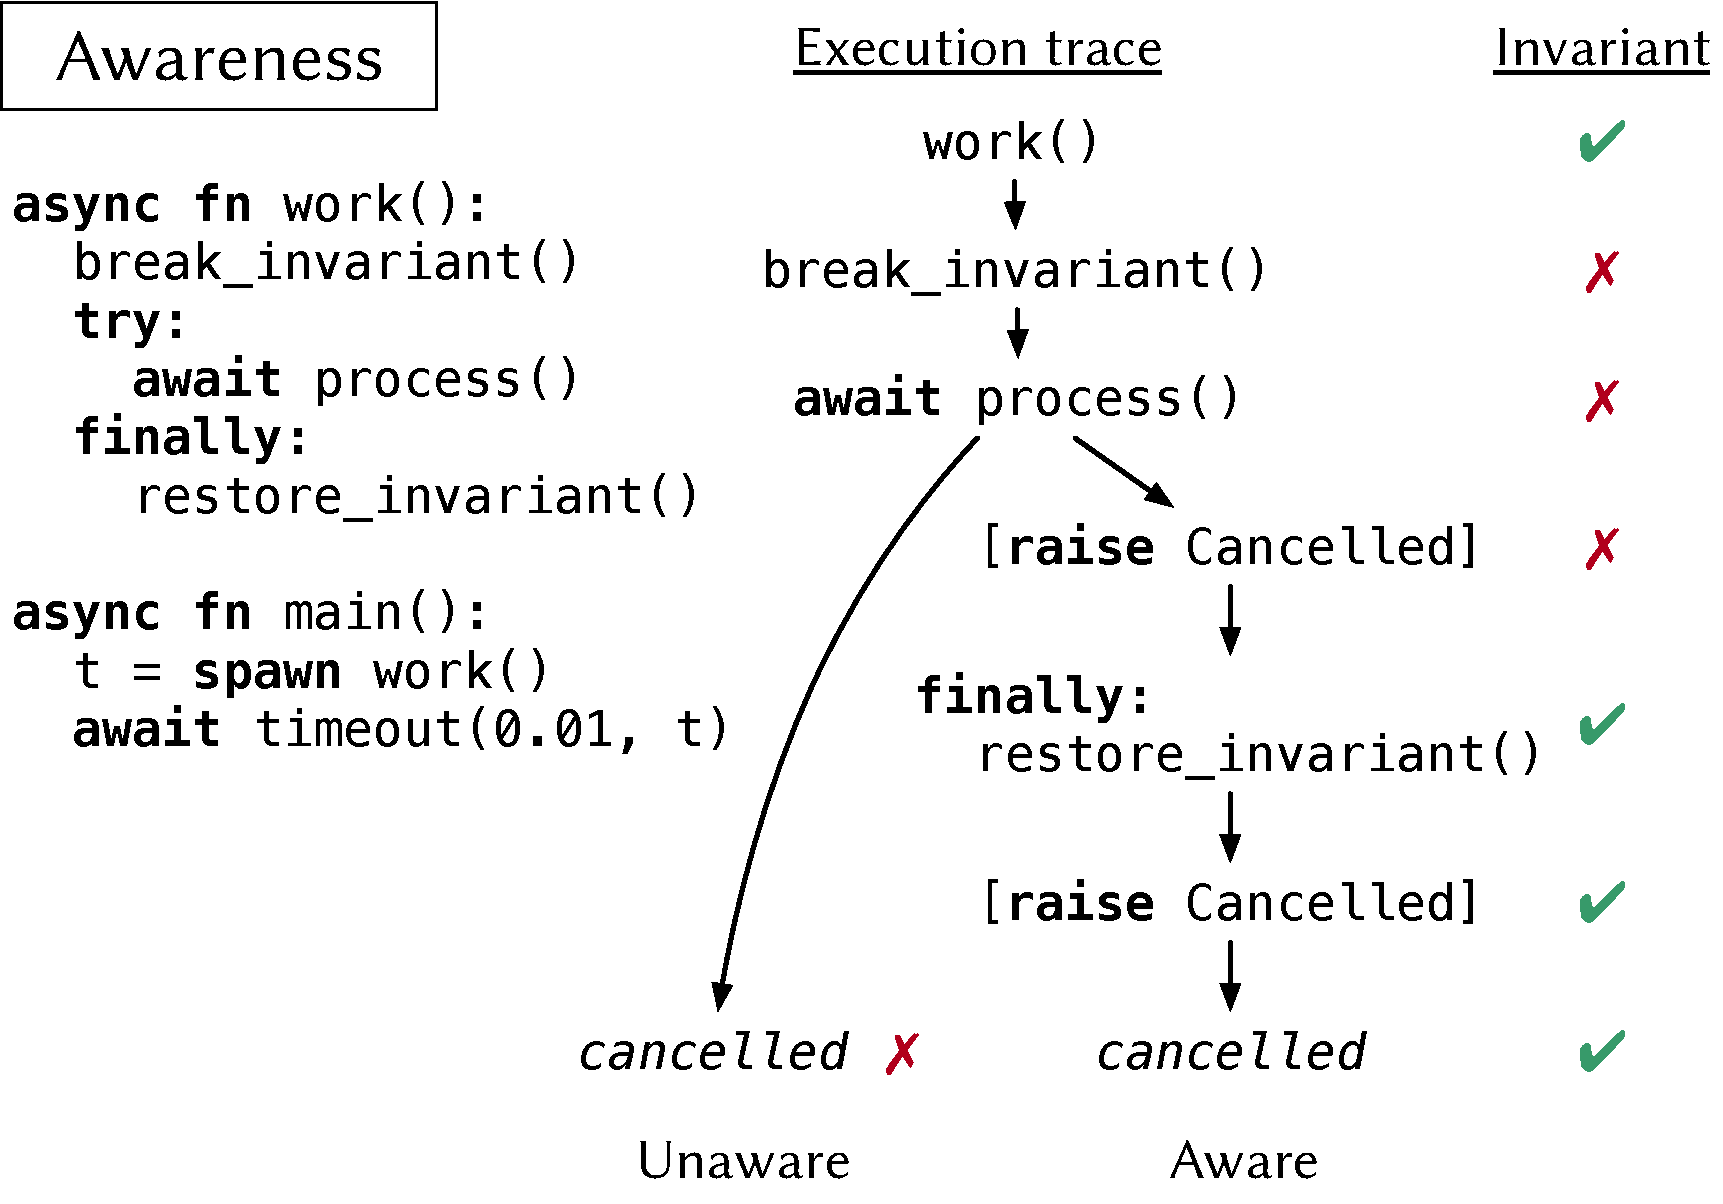
\includegraphics[width=\linewidth]{f/cooperation.pdf}
  \caption{An example program demonstrating the \Cooperation dimension.}
  \label{fig:cooperation}
% \end{figure*}
\end{wrapfigure}

The most straightforward approach is \emph{unaware} cancellation, where a task has no opportunity to react to being cancelled. This approach is taken by Rust in both Tokio and Smol. In Rust, cancellation essentially means never executing a coroutine again after it has yielded. With a direct handle on the coroutine, this simply means not polling the coroutine, or explicitly dropping it. If the coroutine is within a task, then the task must be marked as cancelled, and the runtime will similarly refuse to reschedule the task.

By contrast, Python and Swift both implement a form of \emph{aware} cancellation. In Python (both Asyncio and Trio), when a task is cancelled, a cancellation exception is thrown into the task. An async function can wrap any await point in a try/except block which can catch this cancellation exception, performing cleanup or consuming the exception.
%
In Swift, when a task is cancelled, a flag is set indicating that the task is cancelled. Functions can then opt-in to raising a cancellation exception when this flag is set.

\paragraph{Design rationale.} A benefit of unaware cancellation is that tasks can be reliably cancelled. The principal case that delays unaware cancellation is a compute-bound task which does not cooperatively yield to the runtime. With aware cancellation, functions can either ignore cancellation or fail to opt-in, which we discuss further in \Cref{ssec:designdims:direction}.

A major drawback to unaware cancellation is that cancellation can easily violate logical invariants of a program. For example, consider the program in \Cref{fig:cooperation}. Say a program wants to do asynchronous work in a critical region where an invariant is broken and later restored. With unaware cancellation, the \code|work| task can be halted at \lstinline[language=Pseudo]|await process()|, causing the invariant to remain broken. In Rust, this is a widely-documented problem with its cancellation system\footnotemark~\cite{paharia_400_2025,paharia_cancelling_2025}. With aware cancellation through exceptions, the \lstinline[language=Pseudo]|finally| block has the opportunity to restore the invariant before continuing to raise the cancellation exception. 

\cprotect\footnotetext{It is possible in Rust to implement something similar to the \lstinline[language=Pseudo]|finally| block using the \code|Drop| trait. When a task is cancelled, the task is eventually dropped and drop handlers are invokes for all coroutines in the task. One can theoretically define a custom \code|Drop| implementation for a bespoke type that calls \code|restore_invariant|. However, this approach is verbose (requiring a newtype and impl), unwieldy (requires mutable references to data structures, complicating ownership), and synchronous-only (one cannot call async code in a \code|Drop| implementation without blocking.) }
